\documentclass[12pt]{beamer}
\usetheme{Boadilla}
\usepackage{graphicx}
\usepackage{algorithm2e}
\graphicspath{{images/}}
\title{CMPT 155: Computer Applications for Life Sciences}
\subtitle{Lecture 5: Formulas and Functions}
\author{Ivan E. Perez}
\institute{}
\date{January 26, 2022}
\usepackage{booktabs} % Allows the use of \toprule, 
\usepackage{appendix}
\usepackage{enumerate,multicol}
\usepackage{amsmath, amssymb, amsthm}
\usepackage{tikz}
\usepackage{amsxtra}
\begin{document}
	
	\begin{frame}
		\titlepage
	\end{frame}
	
	\begin{frame}
		\frametitle{Presentation Outline}
		\tableofcontents
	\end{frame}
	\section{Creating Basic Formulas}
	
	\begin{frame}
		\frametitle{Creating Basic Formulas}
		\begin{itemize}
			\item A formula is a series of instructions that are placed in a cell to perform a calculation.
			\item Formulas must begin with an equal sign `=' (e.g., =1+1).
			\item try the example and see what Excel returns.
		\end{itemize}
	\end{frame}

	\begin{frame}
		\frametitle{Arithmetic Operators}
		\begin{center}
			\begin{tabular}{llll}
				Operator & Name & Example & Return\\
				\hline
				$+$ & Addition & $=1+1$ & $2$ \\
				$-$ & Subtraction & $=1-1$ & $0$ \\
				$*$ & Multiplication& $=2*2$ & $4$ \\
				$/$ & Division & $=4/2$ & $2$\\
				$\sphat$ & Exponentiation&  $=2 \sphat 3$ & $8$ \\
				$\%$ & Percent & $=20\%$ & $0.20$
			\end{tabular}
		\end{center}
	\end{frame}

	\begin{frame}
		\frametitle{Excel's Order of Precendence}
		Excel's order of precedence differs a little from traditional PEMDAS. 
		\begin{enumerate}
			\item Parentheses
			\item Percent
			\item Exponents
			\item Division \& Multiplication
			\item Addition \& Subtraction
		\end{enumerate}
		While order of precedence is important, reduce ambiguity by adding parentheses around terms you think can be affected by order of precedence.\\
		\bigskip
		Try these examples to see how excel chooses to modify order of operations.
		\begin{itemize}
			\item $= 5+2 * 2 \sphat 3 - 1$
			\item $= 5+2 * 2 \sphat (3-1)$
		\end{itemize}
	\end{frame}
	\begin{frame}
		\frametitle{Cell References}
		We can refer to values in other cells by using cell references. \bigskip 
		\begin{exampleblock}{Outcome from refering to cells}
		Suppose Cell A1 contains the value 1. What value would be returned if we wrote $ = \texttt{A1} + \texttt{A1}$ in a new cell?
		\end{exampleblock}
		\bigskip
		We can use autofill to solve a sequence of equations. try using autofill on a formula that contains call references to see how the funciton changes.
\end{frame}
\section{Exercises}
	\begin{frame}
		\frametitle{Exercise 1}
			\begin{enumerate}
				\item Download \textit{Llama\_Caloric\_Intake.xlsx}
				from moodle. 
				\item Insert a formula in cell E2 to calculate how much the \textit{caloric intake} is \textbf{per} \textit{body weight}.
				\item Autofill the formula to the end of the list.
				\item Format the data in Column E to keep to 4 decimal places. 
				\item Add the title ``Intake per Body weight"  to Column E. 
			\end{enumerate}
	\end{frame}
	\begin{frame}
		\frametitle{Exercise 1: Solution}
		\begin{center}
		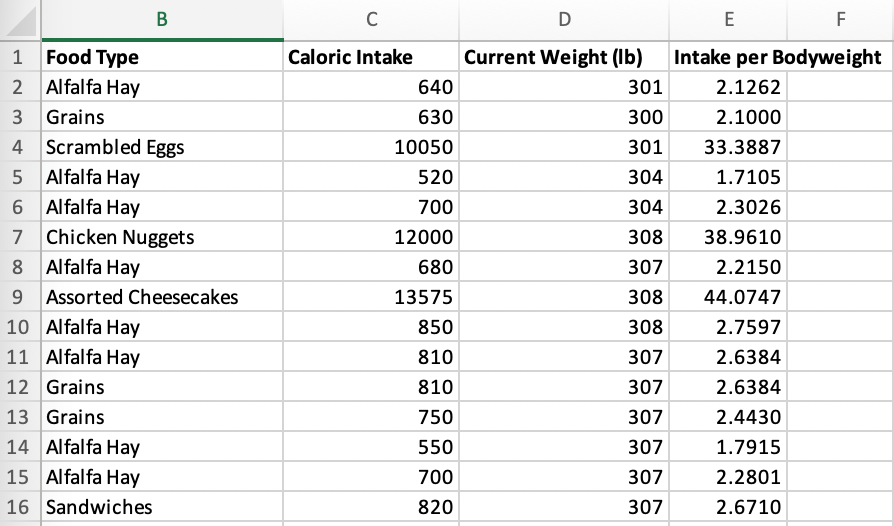
\includegraphics[width= 0.6 \textwidth]{Exercise1Soln.png}
		\end{center}
	Explanation:\begin{enumerate}
		\item  in Cell E2 type $=\texttt{C2} / \texttt{D2}$
		\item Autofill the formula to cell E16.
		\item Select cells E2:E16 and right click the selection
		\item click on Format Cells.
		\item Change the cell format tonumber and change decimal places from 2 to 4. 
		\end{enumerate}
	\end{frame}
	\begin{frame}
		\frametitle{Exercise 2}
		\begin{enumerate}
			\item Download \textit{StudentGrades1.xlsx}
			\item Calcualte the final mark for each student.
		\end{enumerate}
	\end{frame}
	\begin{frame}
		\frametitle{Exercise 2: Solution}
		\begin{center}
			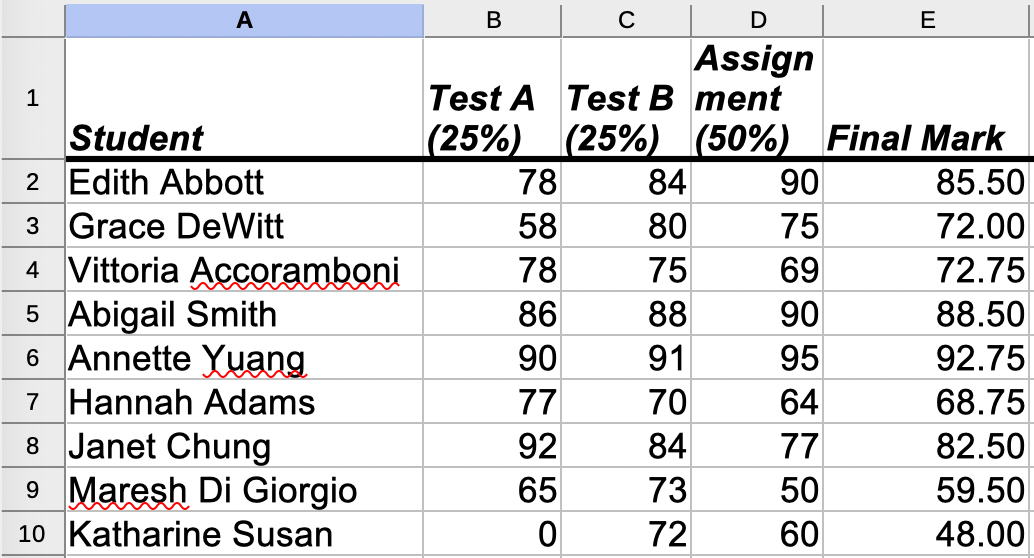
\includegraphics[width= 0.6 \textwidth]{Exercise2Soln.png}
		\end{center}
		\begin{enumerate}
			\item Select cells B2:E10.
			\item If in the home tab of the ribbon go to Number tab andchange the number back to general from percent. 
			\item Calculate the weighted average for the Edith Abbot's scores in E2 using appropriate cell references. 
			\item it should read $=(\texttt{B2}*0.25)+(\texttt{C3}*0.25)+(\texttt{D3}*0.5)$
			\item Use autofill to fill in scores for successive students.		
		\end{enumerate}
	\end{frame}
\section{Cell Ranges}
	\begin{frame}
		\frametitle{Cell Ranges}
		\begin{itemize}
			\item Comma (,)
				\begin{itemize}
					\item separates more than one cell/cell range. 
					\item e.g., A1, B7, H9
					\item Also used to separate arguments in functions.
				\end{itemize}
			\item Colon(:)
				\begin{itemize}
					\item use to describe selections solely by the top-left and bottom-right corners of a block of cells. 
					\item e.g., A1:A5, A2:B3
				\end{itemize}
		\end{itemize}
		\begin{figure}[htb]
		\begin{minipage}[t]{0.32\linewidth}\centering
			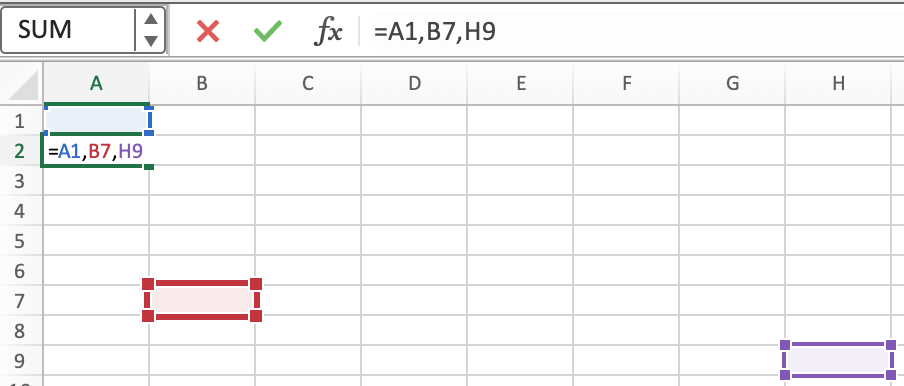
\includegraphics[width=0.9\linewidth]{selection1.png}
			\medskip
			\centerline{(a)}
		\end{minipage}\hfill
		\begin{minipage}[t]{0.32\linewidth}\centering
			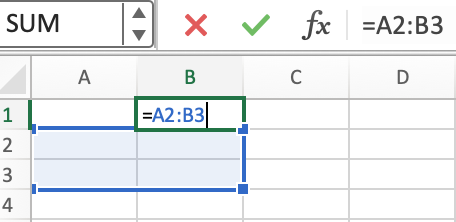
\includegraphics[width=0.9\linewidth]{selection2.png}
			\medskip
			\centerline{(b)}
		\end{minipage}
	\begin{minipage}[t]{0.32\linewidth}\centering
		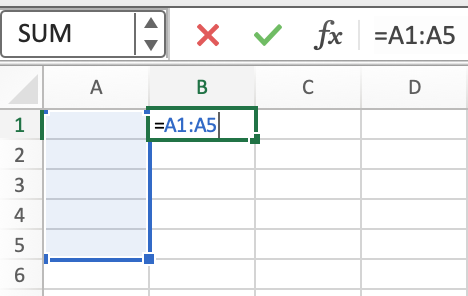
\includegraphics[width=0.9\linewidth]{selection3.png}
		\medskip
		\centerline{(c)}
	\end{minipage}
	\caption{different selections for examples above}
	\end{figure}
	\end{frame}
	\begin{frame}	
		\frametitle{Cell Ranges (cont.)}
		\begin{itemize}
				\item Selecting entire rows is done by writing the row number twice separated by a colon, (e.g., 2:2)
				\item Selecting entire columns is done by writing the column letter twice (e.g., B:B)
		\end{itemize}
		\begin{figure}
			\begin{center}
				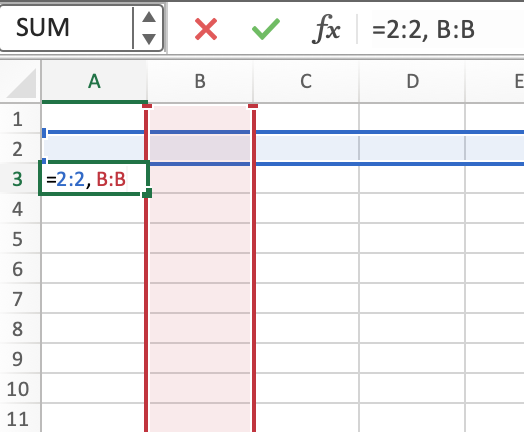
\includegraphics[width=0.4\textwidth]{rowcolumnselection.png}
			\end{center}
			\caption{selection range in 	examples above}
		\end{figure}
	\end{frame}
\section{Functions and Formulas}
	\begin{frame}
		\frametitle{The SUM() function}
		\begin{itemize}
			\item inputs : sequence of cells or selections that may contain numerics.
			\item outputs : single value output summing values in the selection. 
		\end{itemize}
	\begin{figure}
		\begin{center}
			\includegraphics[width=0.5\textwidth]{SUMex.png}
		\end{center}
		\caption{Example of SUM() Function}		
	\end{figure}
	\end{frame}
	\begin{frame}
		\frametitle{Example: Profit Analysis}
		\begin{enumerate}
			\item Download \textit{ProfitAnalysis.xlsx}
			\item Use SUM() to compute totals in cells B7:D7.
			\item Use SUM() and `/' compute the average in cells E4:E7. 
		\end{enumerate}
		\begin{figure}
			\begin{center}
				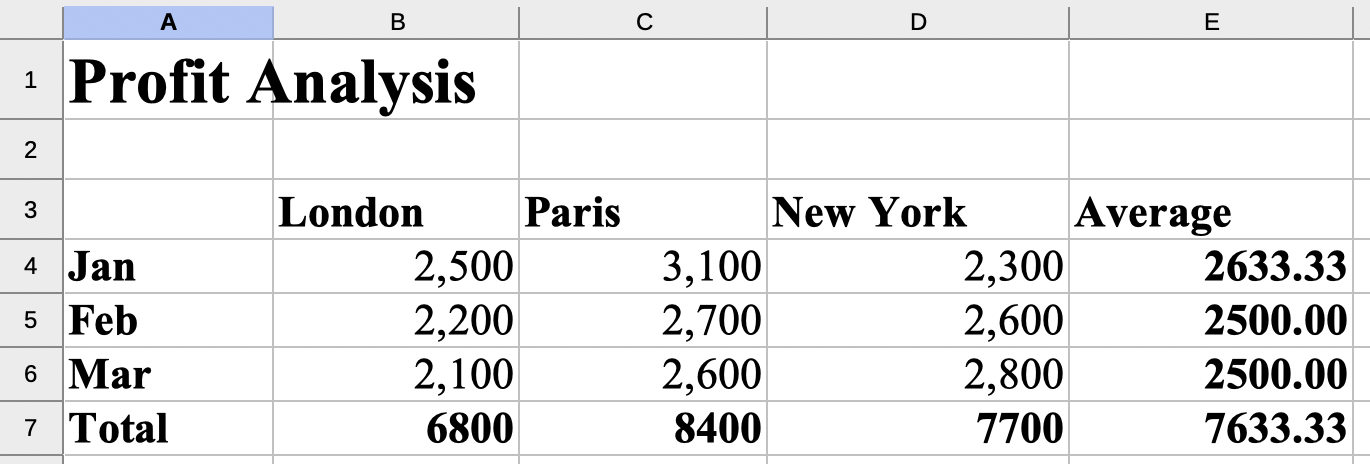
\includegraphics[width=0.5\textwidth]{ProfitAnalysisEx.png}
			\end{center}
			\caption{Profit Analysis Solution}
		\end{figure}
	\end{frame}

	\begin{frame}
		\frametitle{The AVERAGE() function}
		\begin{itemize}
			\item The AVERAGE() function takes arithmetic means(i.e., simple average) of a selection.
			\item The average function will compute averages of numerics but will ignore cells that contain text/strings or blanks.
		\end{itemize}
	\bigskip
	Try:
	\begin{enumerate} 
		\item doing the Profit Analysis example using AVERAGE(). 
		\item deleting and see how the computed average changes.  
	\end{enumerate}
	\end{frame}
\section{Testing/Error Analysis}
	\begin{frame}
		\frametitle{Types of Errors}
		When learning how new functions and operators work, take time to break them and understand their limitations. 
		When entering functions you may run into these kinds of error messages
		\begin{tabular}{ l | l | l }
			Error Code &  Type &Description \\
			\hline
			\#\#\#\#\ & None & The number returned was too long. Expand \\
			&& the column width to see the number. \\
			\#NAME! & Name & Excel does not recognize the \textbf{Name} of\\
			 && the function you have typed.\\
			\#VALUE! & Value & You have entered a \textbf{Value} for the cell that \\
			&& does not work with the operator. \\
			\#DIV/0! & Division & Somehow you attempted to divide by 0. \\
			\#NULL! & Null & When you forget to separate two cell\\
			&& references. \\
			\#REF! & Reference & The Cell contains incorrect references to\\
			&& other cells. \\
		\end{tabular}
	\end{frame}
	
\end{document}

% things to do 
% pics replace, notes




